\documentclass[main.tex]{subfiles}
\begin{document}

\section{Prewriting} 
\label{sec:prewriting}

\begin{frame}[fragile]{Example Problem - Pumpkin Launch}
	\begin{itemize}
		\item Let's make a device to help us calculate the max distance and height
				our pumpkin will travel
		\item Depends on the launch angle: 
			\[ 
				\vec{r_o} = \vec{0} , 
				\vec{v_{o}} = 
					\begin{bmatrix} \cos{\theta} \\ \sin{\theta} \end{bmatrix} 
			\]
		\item Max height: 
			\[
				\begin{bmatrix}
					   0 & \frac{v_{o_{x}}}{g}
					\\ 0 & \frac{v_{o_{y}}}{2 g}
				\end{bmatrix}\vec{v_0}
			\]
		\item Max distance: \[d = \frac{2 v_{o_{x}} v_{o_{y}}}{g}\]
	\end{itemize}
	
	% subsection pumpkin_launch_ (end)
\end{frame}

\begin{frame}{Prewriting}
	\begin{itemize}
		\item Plan how you'll go from math to code: psuedocode
		\item Write out algorithms.
		\item Develop program execution sequence.
	\end{itemize}
\end{frame}

%\begin{frame}[fragile]{Prewriting: Psuedocode}
	%\begin{itemize}
		%\item Use block Diagrams: 
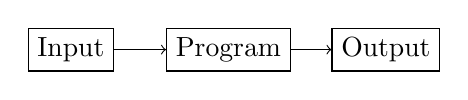
\begin{tikzpicture}
	\node[draw,rectangle] (in) at (0,0) {Input};
	\node[draw,rectangle] (prog) at (2,0) {Program};
	\node[draw,rectangle] (out) at (4,0) {Output};

	\draw[->] (in) -- (prog);
	\draw[->] (prog) -- (out);
\end{tikzpicture}

		%\item Use psuedocode: 
			%\begin{algorithmic}
				%\STATE $S \leftarrow \text{Get INPUT}$
				%\STATE $\text{OUTPUT} \leftarrow \text{Program } S$
				%\RETURN OUTPUT
			%\end{algorithmic}

	%\end{itemize}
%\end{frame}


\end{document}
